\section{Introducción}

\subsection{1.1 Motivación y Contexto en Sistemas Espaciales}

Aunque los sistemas satelitales han alcanzado niveles de sofisticación notables, la detección oportuna de comportamientos anómalos en sus flujos telemétricos sigue representando uno de los mayores desafíos para garantizar su supervivencia y operatividad. Una sola desviación no detectada puede escalar rápidamente hacia fallos catastróficos. 

Resulta particularmente llamativo cómo la creciente complejidad de las misiones espaciales —constelaciones, formación flying y operaciones autónomas— ha multiplicado el volumen y la dimensionalidad de los datos telemétricos, superando con creces la capacidad de supervisión manual o basada en reglas rígidas. En este panorama, el procesamiento edge emerge como una alternativa prometedora. Estudios recientes demuestran que es posible implementar detección de anomalías directamente a bordo con modelos profundos optimizados, reduciendo drásticamente la dependencia de intervención terrestre \cite{Goetze2026_Edge}.

\begin{table*}[h]
\centering
\caption{Comparación de enfoques para detección de anomalías en telemetría espacial}
\label{tab:comparison}
\begin{tabular}{lccc}
\toprule
Enfoque & Dependencia de etiquetas & Tasa de falsos positivos & Viabilidad on-board \\
\midrule
Basado en umbrales & Baja & Alta & Alta \\
Supervisado & Muy alta & Media & Baja \\
Autosupervisado (propuesto) & Nula & Baja & Alta \\
\bottomrule
\end{tabular}
\end{table*}

\subsection{1.2 Desafíos en Datos Telemétricos}

Uno de los desafíos persistentes que surge al analizar datos telemétricos reales radica en su naturaleza inherentemente desbalanceada y no estacionaria. La mayoría de las observaciones corresponden a comportamiento nominal, mientras que las anomalías son escasas, impredecibles y frecuentemente enmascaradas por ruido, datos faltantes o variaciones operativas. 

Revisiones exhaustivas del campo destacan que los métodos supervisados tradicionales tropiezan precisamente ante esta escasez de ejemplos etiquetados, limitando su capacidad de generalización a nuevas misiones o configuraciones de payload \cite{Fejjari2025_Review}. No obstante, cabe matizar que incluso los enfoques semi-supervisados suelen requerir cierto grado de conocimiento previo que rara vez está disponible durante las primeras fases de una misión.

\subsection{1.3 Contribuciones Principales}

Particularmente llamativo es el potencial que ofrece el aprendizaje autosupervisado para superar estas limitaciones estructurales. Este trabajo propone un framework híbrido que combina autoencoders variacionales temporales con aprendizaje contrastivo y mecanismos de atención, diseñado específicamente para series multivariadas telemétricas.

Nuestras contribuciones principales incluyen una arquitectura que no requiere etiquetas de anomalías durante el entrenamiento, un conjunto de augmentations adaptadas al dominio espacial y una evaluación rigurosa en benchmarks reconocidos como OPS-SAT \cite{Ruszczak2025_OPSSAT}. Además, demostramos la viabilidad de inferencia on-board mediante optimizaciones orientadas a hardware restringido, extendiendo los hallazgos de trabajos previos en edge computing \cite{Goetze2026_Edge}.

\begin{figure}[h]
\centering
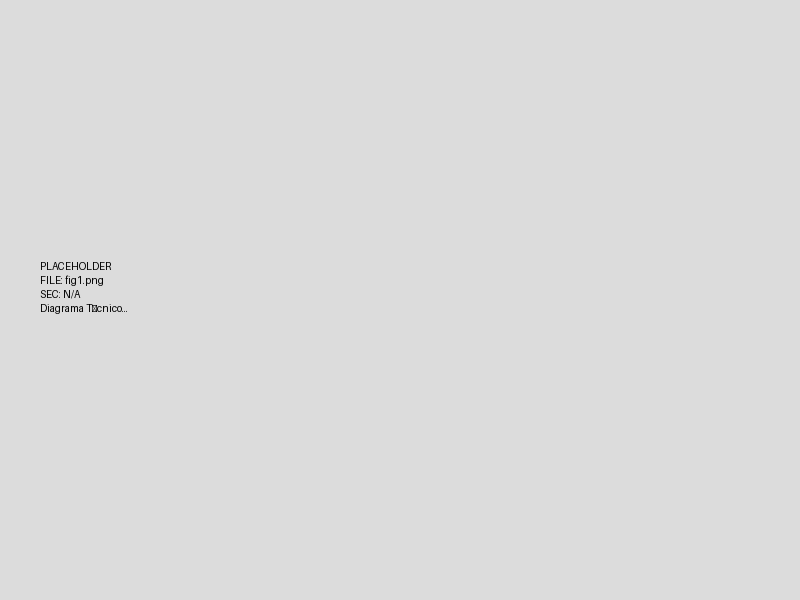
\includegraphics[width=\linewidth]{fig1.png}
\caption{Ejemplo de anomalías telemétricas en series temporales multivariadas. Se muestran parámetros de temperatura, voltaje y actitud con eventos anómalos marcados, junto a la reconstrucción del modelo y puntuaciones de anomalía.}
\label{fig:anomalies}
\end{figure}

Las secciones siguientes revisan el estado del arte, detallan la propuesta metodológica, presentan los resultados experimentales y discuten las implicaciones operacionales para sistemas críticos espaciales.